\documentclass[10pt,twocolumn]{article}

% use the oxycomps style file
\usepackage{oxycomps}
\usepackage{listings}
\usepackage{xcolor}
\usepackage{geometry}
\usepackage{graphicx}
\usepackage{caption}

% Define custom colors for code listings
\definecolor{codegreen}{rgb}{0,0.6,0}
\definecolor{codegray}{rgb}{0.5,0.5,0.5}
\definecolor{codepurple}{rgb}{0.58,0,0.82}
\definecolor{backcolour}{rgb}{0.95,0.95,0.92}

% Define code listing style
\lstdefinestyle{mystyle}{
    backgroundcolor=\color{backcolour},
    commentstyle=\color{codegreen},
    keywordstyle=\color{magenta},
    numberstyle=\tiny\color{codegray},
    stringstyle=\color{codepurple},
    basicstyle=\footnotesize\ttfamily,
    breakatwhitespace=false,
    breaklines=true,
    captionpos=b,
    keepspaces=true,
    numbers=left,
    numbersep=5pt,
    showspaces=false,
    showstringspaces=false,
    showtabs=false,
    tabsize=2
}

% usage: \fixme[comments describing issue]{text to be fixed}
% define \fixme as not doing anything special
\newcommand{\fixme}[2][]{#2}
% overwrite it so it shows up as red
\renewcommand{\fixme}[2][]{\textcolor{red}{#2}}
% overwrite it again so related text shows as footnotes
%\renewcommand{\fixme}[2][]{\textcolor{red}{#2\footnote{#1}}}

% read references.bib for the bibtex data
\bibliography{references}

% include metadata in the generated pdf file
\pdfinfo{
    /Title (Random Table-top Game Map Generator)
    /Author (Victor Zhu)
}

% set the title and author information
\title{Random Table-top Game Map Generator}
\author{Victor Zhu}
\affiliation{Occidental College}
\email{hzhu@oxy.edu}

\begin{document}

\maketitle



\section{Introduction}

In the community of tabletop role-playing games, DM(Dungeon Master) or Game Runner can be a very tedious job. They must create the game, the adversary, the obstacles, and the reward. So, a random map generator that can randomly create a map with monsters, loots, and NPCs would be really helpful. One of my scripts will create a randomized map, and Another generator will generate a random boss room layout. These will make both DM and players' gaming experience much easier than before.    

Creating immersive and engaging game environments has long been a central pursuit for me. A fundamental aspect of such environments is the intricately designed maps that provide players with a sense of place, adventure, and mystery. A sophisticated and innovative tool - a Random Dungeon and Boss Map Generator- is developed in this pursuit.

I have developed a Random Dungeon and Boss Map generator: the Dungeon Map and the Boss's Map. These maps result from two separate algorithms, each playing a crucial role in enhancing the gaming experience.
The first algorithm I created, Dungeon Map Generator, was inspired by the algorithm "Drunkyard's Walk." The drunkard in the Drunkyard's namesake. takes inspiration from the unpredictable movements of an intoxicated individual. This algorithm introduces an element of randomness and unpredictability to the generated maps, adding an exciting element of surprise for players. My algorithm is different than the generic Drunkyard's walk. I will explain it in more detail in the method.
The second algorithm I designed is a random boss room generator- it gives more constraints than the random dungeon map generator. These algorithms ensure the maps are rich in detail and logic, providing players with immersive and engaging environments to explore.

\section{Problem Context}

Tabletop role-playing games (RPGs) have long captivated players' imaginations, offering rich narratives and immersive experiences. At the heart of these games lies the Dungeon Master (DM) or Game Runner, a dedicated individual responsible for crafting the game world, guiding players through adventures, and orchestrating the story. However, one undeniable challenge that DMs face is the extensive time commitment required for preparation before each gaming session. On average, DMs dedicate 3 to 10 hours per week\cite{quora_dnd_duration} \cite{reddit_dnd_prep}to prepare for a single gaming session, a substantial investment that can often deter individuals from taking on this pivotal role.
Recognizing the significance of this issue, I have started a project aimed at alleviating the preparation burden borne by DMs. The core objective of this project is to provide a practical and efficient tool that streamlines the preparation process, thereby enabling DMs to dedicate more time to enjoying the game and fostering engaging experiences for players.
This project's societal context is integral to understanding its value and impact. Tabletop RPGs serve as a source of entertainment and facilitate social interaction, creativity, and critical thinking. In a world where digital screens often dominate leisure time, tabletop RPGs offer a unique and valuable analog experience that fosters face-to-face communication and collaboration. By reducing the preparation time for DMs to less than 30 minutes, this project seeks to lower barriers to entry, making it more accessible for individuals to take on the role of a DM. The project promotes the growth of tabletop gaming communities, enriching social connections and encouraging creative storytelling.
Moreover, the benefits of this project extend beyond leisure and recreation. The project aligns with the broader trend of leveraging technology to enhance traditional gaming experiences. It reflects a broader societal shift towards innovation, efficiency, and accessibility, aligning with the digital age's demands for streamlined processes and user-friendly tools.
 In a broader societal context, it aligns with the increasing integration of technology into leisure activities, catering to modern society's evolving needs and expectations. Ultimately, this project stands to make a valuable contribution to both the gaming community and the broader social landscape, where the pursuit of shared experiences and creative expression is highly prized.


\section{Technical Background}

In this section, I will briefly touch on the technical background of the code for generating DND boss room layouts and introduce Drunkard's Walk algorithm for context. The Random Dungeon Map Generator code operates based on predefined room types and constraints, adhering to placement rules and validating room assignments. It ensures a balanced and thematic layout within a grid-based environment, enhancing tabletop role-playing game experiences. On the other hand, Drunkard's Walk algorithm is a more straightforward yet versatile method for generating random patterns within grids, widely applicable in various procedural generation tasks. These technical insights provide a foundation for understanding the code's functionality and relationship to established algorithms in procedural generation.
 
The code for Random Boss Map Generator code generates a "boss" room layout on a grid. It defines various room types with maximum counts, follows the rules for room placement (e.g., Throne Room far from Entrance), checks for valid placements based on criteria, and fills the grid with rooms. Matplotlib is used for visualization, displaying each room type in distinct colors. This code streamlines the creation of thematic and balanced boss room layouts for tabletop RPGs.

The Drunkard's Walk algorithm is a straightforward yet effective method for generating random paths or patterns within a grid or space. Starting from an initial point, it repeatedly takes random steps in various directions, recording the visited locations to create meandering or branching paths. Widely used in procedural generation tasks, it can produce diverse and unpredictable outcomes, making it valuable for generating mazes, cave systems, or natural features like rivers and roads. The algorithm's simplicity and adaptability make it popular for creating intricate and randomized structures in various applications.


\section{Prior Work}

The methods of Creating Procedurally Generated Dungeons are various and diverse, each contributing to the dynamic landscapes of digital and tabletop gaming. This section delves into the historical context and evolution of procedural dungeon generation, outlining key methodologies while positioning the current project within this broader spectrum of prior work.

The genesis of procedurally generated dungeons can be traced to the domain of tabletop role-playing games (RPGs), with "Dungeons & Dragons" being a seminal influence. Early RPGs utilized random tables to determine dungeon layouts, room contents, and encounters, imbuing each gameplay session with a sense of unpredictability and adventure. This concept of procedural generation was later adopted and refined within the realm of video games, marking a significant evolution from its tabletop origins. A landmark in this journey was the game "Rogue" (1980), which introduced players to endlessly unique dungeon experiences, setting a precedent for the use of procedural content generation (PCG) in game design.\cite{Holmes2020Rogue}
\begin{figure}
    \centering
    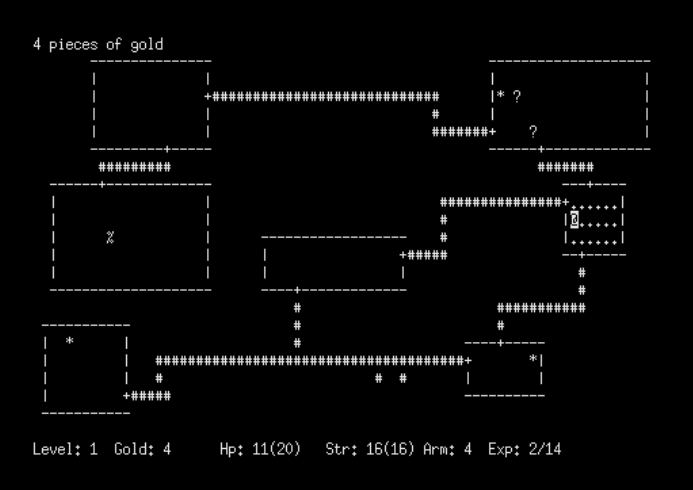
\includegraphics[width=0.5\linewidth]{rougue.PNG}
    \caption{Rougue}
    \label{fig:enter-label}
\end{figure}

As the application of PCG expanded, a variety of algorithms emerged, each suited to different types of games and experiences:

Binary Space Partitioning (BSP): Employed in games like "Doom," BSP generates structured, non-overlapping rooms and corridors, ideal for creating man-made structures.\cite{TwoBitHistory2019DoomBSP}

Cellular Automata: This method, utilized in "Minecraft" for cave systems, excels at creating naturalistic, organic environments through the simulation of cellular evolution.\cite{HeardProceduralDungeonCA}

The choice to adapt the Drunkard’s Walk algorithm was influenced by several factors:

- **Simplicity and Flexibility**: The Drunkard's Walk algorithm is celebrated for its simplicity and flexibility. Unlike BSP, which requires recursive division of space and meticulous planning of rooms and corridors, or Cellular Automata, which depends on evolving rules to generate layouts, the Drunkard's Walk operates on a straightforward premise: move randomly from one point, carving out a path as it proceeds. This simplicity facilitates easy implementation and modification, allowing developers to quickly iterate on dungeon designs without getting bogged down by complex algorithmic constraints.

- ** Unpredictability and Variety **
One of the main advantages of the Drunkard's Walk over BSP is its inherent unpredictability. While BSP generates highly structured and predictable layouts, the random nature of the Drunkard's Walk ensures that each dungeon map is unique, offering a new experience with every generation. This unpredictability can be particularly appealing for games that prioritize exploration and surprise. Unlike Cellular Automata, which also generates varied outcomes, the Drunkard's Walk does not require the relatively "fine-tuning" of rules to achieve desirable results, making it a more straightforward option for generating diverse dungeon layouts.


- **Hardware Efficiency**
Given its straightforward computational process, the Drunkard's Walk is generally more hardware-efficient than its counterparts, particularly for projects where performance is a concern. Cellular Automata, for instance, may require multiple iterations and rule evaluations to generate a final layout, while BSP's recursive space division can be computationally intensive for large maps. The Drunkard's Walk's minimal processing demands make it an excellent choice for projects with limited hardware capabilities or those aiming for scalability across devices.

Ease of Implementation and Experimentation
For developers, especially those working on indie projects or with limited resources, the ease of implementation is a critical factor. The Drunkard's Walk algorithm's simplicity not only makes it accessible for developers with varying levels of experience but also encourages experimentation. Tweaking the algorithm to explore different dungeon layouts or integrating it with other features (like traps, treasures, or enemy placements) can be accomplished with minimal additional complexity.

\begin{figure}
    \centering
    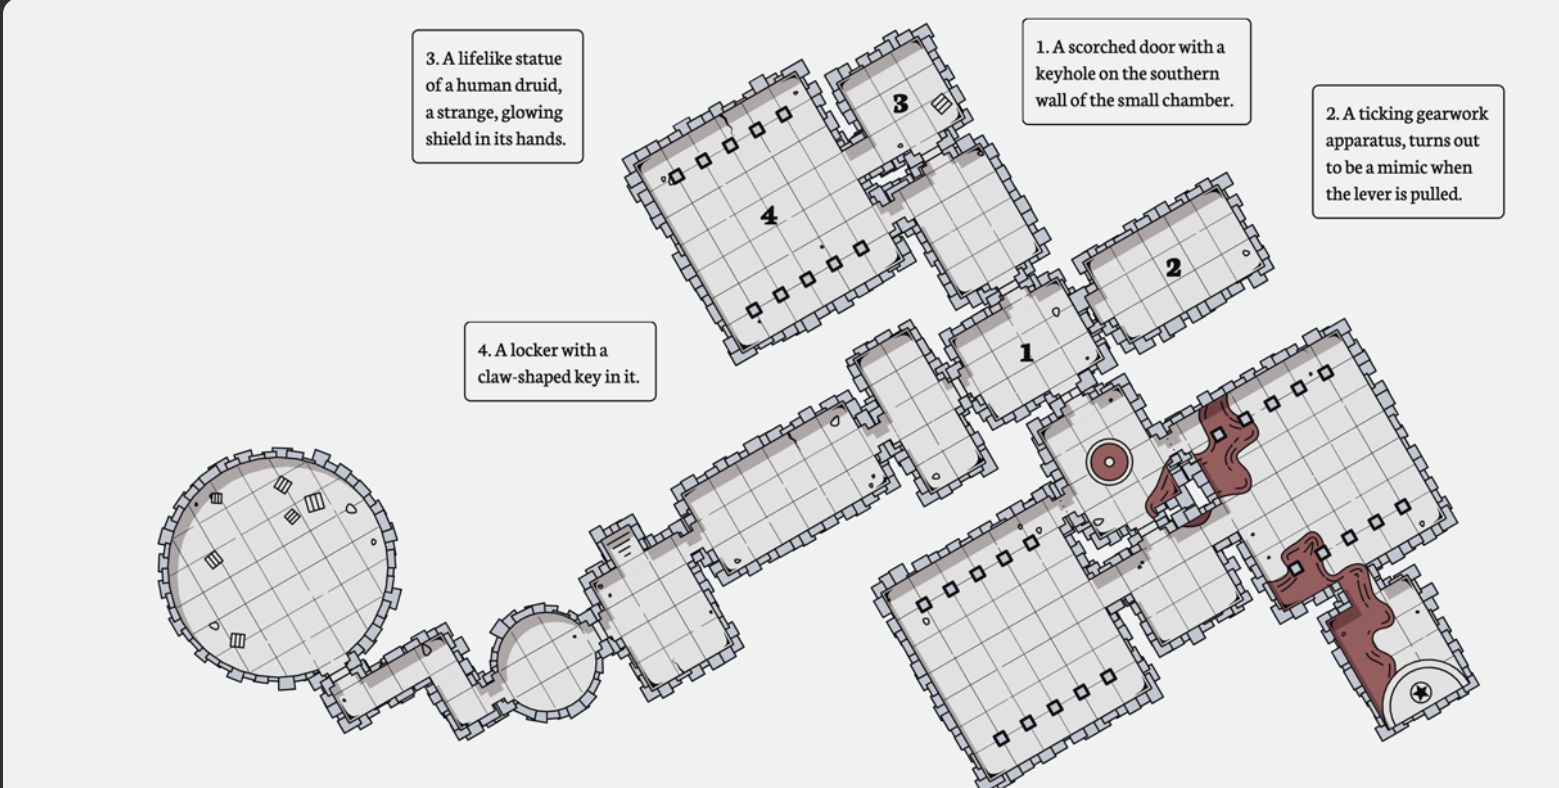
\includegraphics[width=0.5\linewidth]{watab.png}
    \caption{Watabou's Procgen Arcana}
    \label{fig:enter-label}
\end{figure}

I used the Procedural Dungeon Generation: A Drunkard's Walk in ClojureScript as inspiration for my early version of code. The blog post explores procedural dungeon generation using the "Drunkard's Walk" algorithm implemented in ClojureScript. The author discusses the algorithm's basics, where it starts from a point and randomly navigates the grid to create intricate maze-like structures. \cite{jrheard_dungeon_clojurescript}

\begin{figure}
    \centering
    
\includegraphics[width=0.5\linewidth]{mine.png}
    \caption{my output from inspiration from Procedural Dungeon Generation: A Drunkard's Walk in ClojureScript}
    \label{fig:enter-label}
\end{figure}


The post provides insights into the implementation details, including grid initialization, wall generation, and room placement. It also highlights how parameters like randomness and wall density affect the generated dungeons. The blog post offers a practical demonstration of the algorithm's capabilities, showcasing the creation of diverse and engaging dungeon layouts for game development or other applications. However, one of the project's shortcomings is it doesn't guarantee a map for adventure. Sometimes, it looks like a giant opening instead of a dungeon pattern.
Then I found this webpage. It simplifies the drunkard walk algorithm into four steps:
\begin{enumerate}
    \item Pick a random point on a filled grid and mark it empty.
    \item Choose a random cardinal direction (N, E, S, W).
    \item Move in that direction, and mark it empty unless it already was.
    \item Repeat steps 2-3 until you have emptied as many grids as desired.\cite{pcgwiki_drunkardwalk}
\end{enumerate}

It is easy to follow, so I created my algorithm based on this blog.


\section{Methods}
In the development of a procedural map generator for tabletop gaming sessions, feedback was collected from experienced Dungeon Masters (DMs) through online interviews. These DMs, skilled in world-building and game facilitation, highlighted specific areas for enhancement based on their expertise. A recurrent theme was the request for more complex and modular designs for boss rooms, emphasizing the need for these areas to be both visually impressive and narrative-rich. Following initial test plays, the importance of such features became evident, underlining the boss rooms' role in enhancing gameplay and storytelling. Furthermore, one interviewee suggested incorporating extensive details directly onto the maps to reduce the necessity of consulting rulebooks during sessions. Unanimously, all participants expressed a desire for the tool to facilitate a stronger narrative connection among the dungeon's elements, including monsters, obstacles, NPCs, and the overall environment. Consequently, the project was structured into two distinct components: the comprehensive dungeon map and the specialized boss room map, each tailored to address the specific feedback and requirements identified by the DMs.

The initial phase of the procedural map generator's development focused on creating the overall dungeon map. This process began with generating a basic framework consisting of squares connected by lines, with each square designated to represent a room. The assignment of rooms to squares was governed by specific constraints designed to balance gameplay and enhance player experience.

Firstly, a key consideration was maintaining a balanced encounter rate to ensure that players could progress through the game at a reasonable pace. To achieve this, the algorithm was programmed to strategically place stronger encounters adjacent to either weaker encounters or non-combat rooms, such as those containing treasure or traps. This arrangement aimed to moderate the difficulty level, providing players with a mix of challenges and relief.

Secondly, the generator was designed with a reward system to incentivize players. Recognizing that loot is a universal motivator in gameplay, loot drops were programmed to occur with each encounter. Additionally, treasure rooms were strategically placed to follow challenging rooms—either after a trap, a strong encounter, or a boss room—to reward players for their efforts. Puzzle rooms linked to treasure rooms were also incorporated to enhance the sense of achievement from obtaining loot.

The map system was developed with flexibility in mind, allowing Game Hosts to customize the shape and function of rooms according to their preferences. These constraints are fully customizable, providing Game Hosts with the capability to modify them directly in the code to suit their specific needs.

For preset gameplay, the dungeon generator offers three distinct sets of encounters, all within the same underground dungeon theme but varying in difficulty and narrative focus. The "hard" set is combat-oriented, culminating in a dragon as the final boss, while the other sets are geared more towards exploration. This variety allows Game Hosts to tailor the dungeon to the desired type of game session by controlling the probability of each room's generation, thereby enabling them to shape the gameplay experience to match their vision.



\subsection{Separate Programs for Dungeon and Boss Rooms}

In the development of the boss room map, an emphasis was placed on further customization options to meet Game Hosts' specific requests. Recognizing the boss room as not merely the final challenge of a dungeon but also as a pivotal narrative moment, enhancements were made to distinguish these rooms significantly from those in the general map layout. Feedback from interviews highlighted the need for the boss room to encompass a variety of unique spaces beyond the traditional combat arena, including security rooms, additional treasure rooms, kitchens, sleeping quarters, and bathrooms. The inclusion of such rooms aims to humanize the boss character, providing players with a more immersive and nuanced experience by revealing the daily living aspects of the boss's existence within the dungeon.

To structure these immersive environments effectively, specific constraints were applied to the placement of rooms within the boss map. Key requirements included positioning the throne room as far from the entrance as possible to symbolize the culmination of the players' journey through the dungeon. Guard rooms were mandated to be located at the perimeter of the map, serving as the first line of defense. Furthermore, the sleeping area was to be situated adjacent to the throne room, with the bathroom in close proximity, reflecting a logical arrangement of personal spaces. These constraints were designed to ensure a coherent and realistic layout that contributes to the narrative depth and strategic complexity of the final encounter.

Customization remains a cornerstone of the boss room generator, allowing Game Hosts to adapt each area and constraint to their preferences. This flexibility enables the creation of tailored experiences that align with the Game Hosts' vision for their campaign, ensuring that each boss room is not only a challenge but also a story-rich environment that enhances the overall gameplay experience.

\begin{figure}[h]
\centering
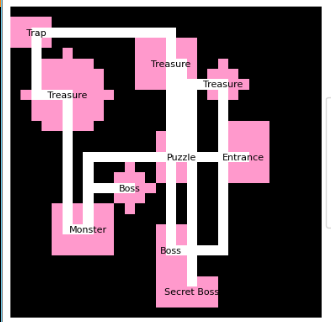
\includegraphics[width=0.5\linewidth]{mymap.png}
\caption{Example of a Random Dungeon Map}
\label{fig:dungeon-map}
\end{figure}

The \textit{Random Boss Room Generator} focuses on spatial hierarchy and thematic placement, influenced by GameHosts' emphasis on the narrative significance of boss encounters. It ensures that crucial rooms are placed logically within the dungeon to build anticipation and challenge.

\begin{figure}[h]
\centering
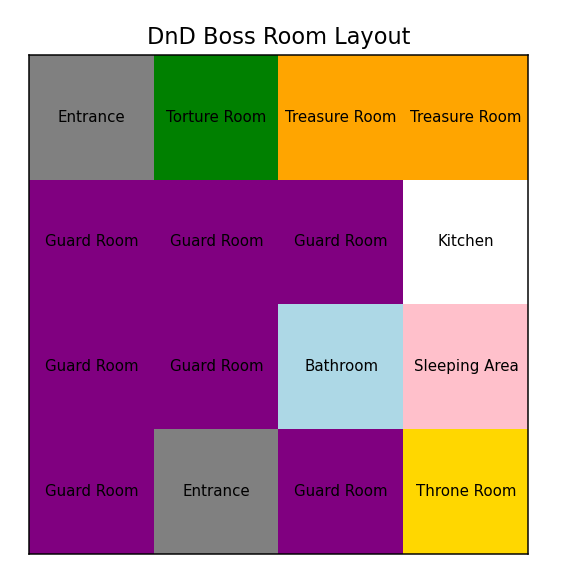
\includegraphics[width=0.5\linewidth]{bossmap.png}
\caption{Example of a Boss Room Layout}
\label{fig:boss-room}
\end{figure}
the game also comes with three pre-set gaming content. Each set of the game contains traps, monsters, and treasure.  When the map is generated, there will be showing monster, trap, and other elements next to the map and provide a description of the element such as how hard the element is, a ,description and loot.  The final boss also is different in each set. One is the hibernating red dragon, one is dark elf siblings, and the final one is the goblin king. Each set of monsters is unique. It is designed so each set of playthroughs is unique, allowing the players to experience new challenges each time they explore the dungeon. The monsters and traps are designed to connect to the theme. These three sets of monsters and traps are set in the theme of the underground dungeons. According to the lore provided in the Monster Manual, most monsters in the set dwell in the underground.   


\section{Evaluation Metrics}

These are the evaluation metrics I created on the first day I designed the project. I think these are suitable for the project.

\begin{enumerate}
    \item \textbf{Good Storyline (Who What Why):}
    
    \textit{Importance:} A good storyline is crucial for engaging players in the game world. It provides context, purpose, and motivation for their actions. A well-crafted narrative can make the gameplay more immersive and enjoyable. Measured through DM and player feedback on the storyline's integration and immersive quality.  \cite{reddit_dnd_campaign_fun}
    
    \item \textbf{Good Adversary (Motivation, Theme, Difficulty, Variation):}
    
    \textit{Importance:} The adversary or antagonist in a game adds challenge and conflict, making the gameplay interesting. Their motivation and theme contribute to the depth of the story. The player will decide is the game has the right amount of difficulty and variation by giving their opinion.\cite{reddit_dnd_campaign_fun}    
    \item \textbf{Good Resolution (Rewarding or not, Meaning):}
    
    \textit{Importance:} The resolution of the hero's journey is what players work toward. A rewarding resolution provides a sense of accomplishment and satisfaction, motivating players to continue or replay the game. The meaning or impact of the resolution can leave a lasting impression on players. This is determined by interviewing both GameHost and players \cite{reddit_dmacademy_oneshot}
\end{enumerate}

A rewarding resolution provides a sense of achievement and closure, motivating players to complete and potentially play the game again.
The importance of these metrics is justified in the context of game design literature, where a compelling narrative, challenging gameplay, and immersive world-building are often considered essential elements for successful games. These metrics help ensure that your algorithm generates game scenarios that are enjoyable, engaging, and memorable for players.
 


\section{Evaluation Results and Discussion}
My methodological approach involved the development of algorithms for procedural dungeon and boss room generation, incorporating feedback from Dungeon Masters (DMs) to ensure the created environments meet gameplay and narrative standards. Initial interviews with five DMs via Discord provided foundational insights that shaped algorithm development. Key focus areas included enhancing narrative depth, ensuring logical room connectivity, and maintaining a balance of challenge and exploration within the generated maps.

\subsection{Evaluation Process and Results}
Good Storyline
        After interviewing GameHost and the players after the playtesting using the dragon preset. The players considered random-generated adventure similar to the past GameHost-designed games. The game host expressed that the characters, monsters, and trap made sense in his playthrough, but he did not think a short game like the pre-set game needed any storyline.

Good Adversary
        The two primary sources of the adversary are the room positions and the pre-set games. The room position is determined by rules, such as the weak monster or treasure following the strong monster, etc. The pre-set game comes with pre-set monsters, traps, and puzzles. The player can go through each challenge in 5 minutes. According to the GameHost, this is a regular time for players to get through a challenge in a human-made game session. As for the players, they reflect that the monsters' puzzles and traps are relatively easy, but they feel like they have faced challenges.    

Good Resolution
        In the end, after the player defeats one of the bosses in the pre-set gameplay, they feel they have defeated a harder enemy.  GameHost also gave the player a conclusion based on defeating the boss dragon. After interviewing the players, they felt satisfied. 


.


\section{Ethical Considerations and Implementation}

\subsection{Fairness and Inclusivity}
\begin{itemize}
    \item : My algorithm generates maps randomly with contraction randomization functions and regularly tests outcomes for bias.
    \item To promote \textbf{inclusivity}, the content generation algorithms were designed to avoid stereotypes and ensure a wide representation of characters and scenarios, fostering a positive gaming environment for all.
\end{itemize}

\subsection{Player Agency}
\begin{itemize}
    \item \textbf{Transparency} about the procedural generation process is provided through documentation and in-game explanations, giving players and DMs insight into how dungeons are created.   Customization options are enabled, allowing GameHosts to modify algorithm parameters to suit their campaign needs, enhancing player agency in shaping their adventure.
\end{itemize}


\subsection{Data Privacy}
\begin{itemize}
    \item \textbf{Data protection} measures are implemented to ensure that any collected data, such as player preferences or custom dungeon settings, are securely stored in the local computer.
\end{itemize}

\subsection{Accountability and Continuous Improvement}
\begin{itemize}
    \item I am committed to \textbf{accountability}, with mechanisms in place for reporting and addressing biases, bugs, or ethical concerns raised by the community.
    \item I engage in \textbf{continuous improvement} by updating algorithms based on player and DM feedback and staying informed about ethical standards within the gaming community.
\end{itemize}

\section{Conclusion}
Through these measures, my project aims to deliver a procedurally generated dungeon and boss room experience that is ethically responsible, inclusive, and enjoyable for the TTRPG community. I believe that considering these ethical aspects is crucial for the sustainable and positive development of gaming technologies.
In conclusion, the project of developing procedural dungeon and boss room generators for tabletop role-playing games (TTRPGs) has yielded promising results, addressing several critical aspects of game design and enhancing the overall player experience. I have focused on creating immersive, balanced, and ethical gaming environments throughout the project. As I reflect on the achievements and challenges encountered during this endeavor, it is clear that procedural generation has the potential to impact TTRPGs significantly and positively.

Key Achievements:
1. **Enhanced Gameplay**: The procedural dungeon generator has successfully created diverse and strategically structured dungeon layouts, offering players a more engaging and challenging experience. Including dynamic room, captions has added depth to storytelling, while the boss room generator has improved narrative coherence and tactical gameplay.

2. **Fairness and Inclusivity**: Ethical considerations have been central to my project, ensuring that generated content is fair, inclusive, and appropriate for diverse audiences. This approach promotes a welcoming and respectful gaming environment.

3. **Player Agency**: By allowing players and Dungeon Masters (DMs) to customize algorithms and adjust parameters,  I have empowered them to tailor their TTRPG adventures to their preferences. Transparency in procedural generation further enhances player agency, fostering a sense of control and immersion.

4. **Content Appropriateness**: The project has prioritized age-appropriate content, trigger warnings, and cultural sensitivity, making TTRPGs accessible and enjoyable for many players. This approach helps prevent potentially uncomfortable or distressing experiences. All the players and the DMs are comfortable with the content I created.

5. **Ethical Considerations**: I have proactively addressed issues related to intellectual property, data privacy, and accountability, ensuring that the project aligns with ethical standards and legal requirements to my players and DMs.
\section{Future Work}
While the project has achieved several milestones, there is ample room for further development and improvement in the field of procedural dungeon and boss room generation for TTRPGs:

1. **Advanced Algorithms**: Future work can explore more sophisticated algorithms to create even more complex and dynamic dungeon layouts. Incorporating decision trees, machine learning, or neural networks may enable generators to adapt to player preferences and behaviors during gameplay.

2. **Multiplayer Integration**: Integrating multiplayer capabilities, allowing multiple players or DMs to collaboratively or competitively create and explore procedurally generated dungeons, can enhance the social aspect of TTRPGs.

3. **Enhanced Graphics and Visualization**: Improving the graphical representation of generated dungeons, potentially through the integration of graphic design software or 3D modeling, can provide a more immersive visual experience.

4. **Natural Language Processing**: Incorporating natural language processing to generate detailed descriptions of rooms, NPCs, and encounters could further enrich storytelling and reduce the need for manually entering room descriptions.

5. **Player Feedback Mechanisms**: Developing systems for players to provide feedback on generated content and gameplay experiences can help fine-tune algorithms and identify areas for improvement.

6. **Expansion into Other TTRPG Systems**: Adapting the procedural generation tools to work seamlessly with various TTRPG systems beyond Dungeons & Dragons, such as Pathfinder or Call of Cthulhu, would broaden the project's applicability.

7. **Educational Applications**: Exploring how procedural generation can be used for educational purposes, such as teaching game design or history through TTRPG scenarios, can open up new avenues for the project.

8. **Dynamic Difficulty Scaling**: Implementing mechanisms that dynamically adjust dungeon difficulty based on player skill, character level, or party composition can create more tailored and challenging experiences.

9. **Storyline Integration**: Integrating procedural generation into overarching campaign storylines, allowing generated content to align more closely with the narrative, can enhance immersion and coherence.

10. **Cross-Platform Compatibility**: Ensuring that the procedural generation tools are compatible with various platforms, including virtual tabletop systems and mobile devices, can broaden their accessibility.

In summary, the project has made significant strides in developing procedural dungeon and boss room generators for TTRPGs, emphasizing fairness, inclusivity, and ethical considerations. The potential for growth and innovation in this field is substantial, offering exciting opportunities to enhance TTRPG experiences for players and DMs. By continuing to refine algorithms, expand capabilities, and embrace emerging technologies, I can look forward to a future where procedurally generated content plays an even more significant role in tabletop role-playing games.


\section{Timeline}

I commenced this project in the second week of the semester, and as I prepared for my initial presentation, I was uncertain about the path to success. In early October, a significant breakthrough occurred when I developed a program based on the Drunkard's Walk algorithm. However, I found this approach to be overly simplistic. Subsequently, in late October, I completed the prototype for my current project. Following a month of coding and refining, I conducted playtesting at the end of November. Additionally, I successfully created a boss room generator, which involved more intricate constraints than the dungeon map generator. Currently, I am in the process of composing this essay

\section{Replication Instructions}
\section{Prerequisites}

Make sure you have the following prerequisites installed on your system:

\begin{itemize}
    \item Python (3.x recommended)
    \item Matplotlib
    \item NumPy
\end{itemize}

You can install Matplotlib and NumPy using pip:

\begin{lstlisting}[language=bash]
pip install matplotlib numpy
\end{lstlisting}
\section{Tutoiral for Dungeonmap.py}
\subsection{Step 1: Clone the Repository (If Applicable)}

If your code is part of a Git repository, clone it to your local machine:

\begin{lstlisting}[language=bash]
git clone <https://github.com/VictorZhudd/senior-comp2.git>
cd <repository_directory>
\end{lstlisting}

\subsection{Step 2: Open the Python Script and make sure bossroom.py is in the folder}

Open the Python script where you've pasted the provided code. Let's call it \texttt{dungeonmap.py}. Since the code will create not only a dungeon map but also a boss room map, the user must find a function called generate\_dnd\_boss\_room\_layout\_v8 in another script. In my package, you can find it in bossroom.py

\subsection{Step 3: Adjust Room Type Chances}

You can customize the chance of different room types appearing by modifying the \texttt{group\_params} list. Each element in this list represents a group of rooms with associated labels, shapes, and chances.

For example, if you want to increase the chance of "Treasure" rooms appearing, change the chance value (between 0.0 and 1.0) in the \texttt{group\_params} list. Here's how:

\begin{lstlisting}[language=Python]
group_params = [
    (['Treasure', 'Puzzle'], ['rectangle', 'rectangle'], [0.8, 1.0]),  # Increase chance for 'Treasure'
    (['Treasure', 'Strong Monsters'], ['rectangle', 'circle'], [0.2, 0.6]),
    # Add or modify other room groups as needed
]
\end{lstlisting}

\subsection{Step 4: Define Custom Colors}

To define custom colors for room visualization, you can modify the \texttt{colors} array and the \texttt{cmap} colormap. The \texttt{colors} array represents the RGB colors for different room types, and the \texttt{cmap} is the colormap that uses these colors.

Here's how to define custom colors:

\begin{lstlisting}[language=Python]
colors = np.array([
    [0, 0, 0],     # Black for walls (-1)
    [0.8, 0.8, 0.2], # Custom color for 'Treasure' rooms (0)
    [1, 1, 1],     # White for paths (1)
])
cmap = ListedColormap(colors)
\end{lstlisting}

You can adjust the RGB values to specify different colors for each room type.

\subsection{Step 5: Customize Room Descriptions}

Customize room descriptions by modifying the \texttt{room\_descriptions} dictionary. Add or modify descriptions for each room type as needed.

Here's an example of custom room descriptions:

\begin{lstlisting}[language=Python]
room_descriptions = {
    'Treasure': [
        'A glittering treasure chest awaits! It contains a valuable gem.',
        'You found a hidden stash of gold coins and jewelry!',
    ],
    'NPC': [
        'You encounter a friendly merchant who offers to trade with you.',
        'A mysterious traveler shares valuable information about the dungeon.',
    ],
    # Add or modify descriptions for other room types
}
\end{lstlisting}

\subsection{Step 6: Specify Room Dimensions and Map Size}

You can specify the dimensions of rooms and the size of the grid by modifying relevant parameters in the code. For example, to change the minimum and maximum room dimensions, modify the following lines:

\begin{lstlisting}[language=Python]
room_width = random.randint(3, 6)  # Change the range as needed
room_height = random.randint(3, 6)  # Change the range as needed
\end{lstlisting}

Also, define the dimensions of the grid by changing the \texttt{width} and \texttt{height} variables:

\begin{lstlisting}[language=Python]
width, height = 30, 30  # Change to your desired map size
\end{lstlisting}

\section{Step 7: Run the Script}

Save your changes and run the script:

\begin{lstlisting}[language=bash]
python dungeonmap.py
\end{lstlisting}
and it should come out likes this:
\begin{figure}
    \centering
    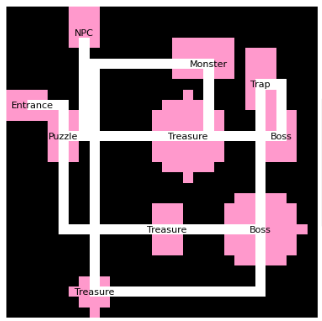
\includegraphics[width=0.5\linewidth]{example1.png}
    \caption{the map part of you result should look like this}
    \label{fig:enter-label}
\end{figure}

\begin{figure}
    \centering
    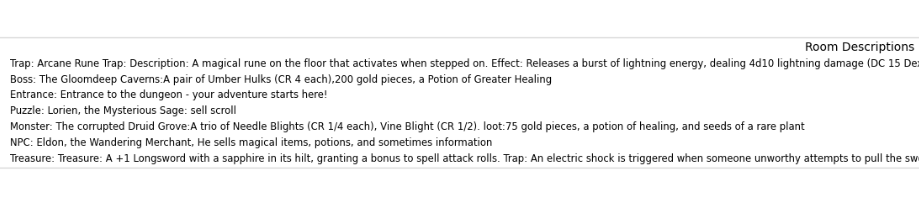
\includegraphics[width=0.5\linewidth]{decs.png}
    \caption{the map should come with these descriptions}
    \label{fig:enter-label}
\end{figure}
it will also trigger bossroom.py and create a boss room map
\section{Tutorial for bossroom.py}
This tutorial provides an interactive guide to enhancing your DnD Boss Room Layout script. It will walk you through the features of the script and demonstrate how to effectively use and modify them to create compelling dungeon designs. This script connects to the dungeonmap.py. It needs both scripts to work.

\subsection{Exploring the Script's Features}
\subsubsection{Creating a Diverse Array of Rooms}
The heart of the script lies in its ability to create various room types. This diversity is managed through a dictionary named \texttt{room\_types}. Here's how to use it:

\begin{itemize}
    \item \textbf{Adding a New Room Type:} To introduce a new room, such as a 'Mystical Study', simply add it to the dictionary with a maximum count. For example:
    \begin{lstlisting}[language=Python]
    room_types["Mystical Study"] = 1
    \end{lstlisting}

    \item \textbf{Changing Room Names:} Modify the keys in the \texttt{room\_types} dictionary to rename rooms.
\end{itemize}

\subsubsection{Customizing the Dungeon Layout}
The layout is represented by a grid, initialized based on a specified size. This grid forms the blueprint of your dungeon. You can easily change the size of the grid to make your dungeon larger or smaller, thus altering the complexity and exploration opportunities.

\subsubsection{Strategically Placing Key Rooms}
The script includes logic for strategically placing important rooms like the Throne Room and the Entrance. You can modify this logic to change the layout dynamics, creating new challenges and narratives.

\subsubsection{Ensuring Logical Room Placement}
The function \texttt{is\_valid\_placement} checks if the placement of a room adheres to the dungeon theme and logic. Modifying this function allows you to set new rules for where specific rooms can be placed.

\subsubsection{Filling the Grid with Adventure}
After setting the key rooms, the script fills in the remaining spaces. This step is crucial for ensuring that every part of your dungeon is engaging. You can modify the filling logic to control the distribution of room types, balancing between challenge and exploration.

the default result should look like this
\begin{figure}
    \centering
    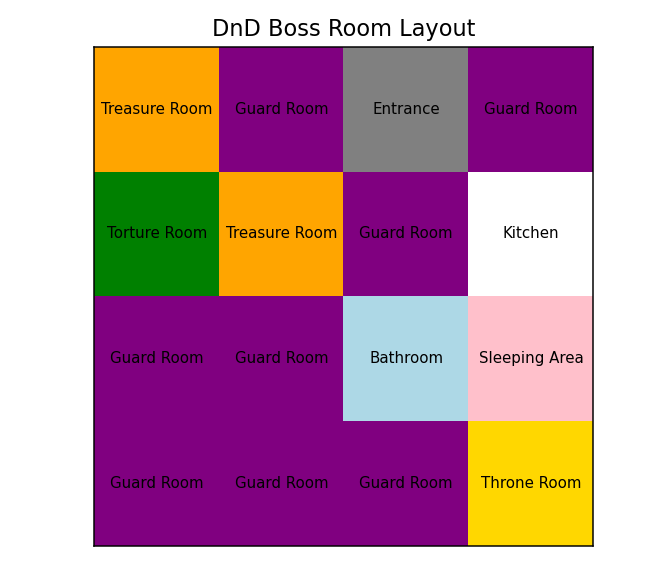
\includegraphics[width=0.5\linewidth]{bossroom.png}
    \caption{default bossroom.py result should look like this}
    \label{fig:enter-label}
\end{figure}
\subsection{Bringing Your Dungeon to Life: A Step-by-Step Example}
Let's go through an example of adding a 'Library' room to your dungeon:

\begin{lstlisting}[language=Python]
# Step 1: Add the Library to room_types
room_types["Library"] = 1

# Step 2: Assign a color to the Library in room_colors
room_colors["Library"] = "saddlebrown"

# Step 3: Modify is_valid_placement for the Library
# Add your custom logic here

# Step 4: Generate the dungeon layout
dnd_room_layout = generate_dnd_boss_room_layout_v8(6)
\end{lstlisting}



\section{Code Architecture Overview}

This section provides a detailed overview of the code architecture for two Python scripts: `bossroom.py` and `dungeonmap.py`. These scripts are designed to generate a Dungeons and Dragons (DND) dungeon layout, including a specific boss room.

\subsection{bossroom.py Overview}
\subsubsection{Purpose}
The `bossroom.py` script is designed to generate a layout for a D\&D boss room. 

\subsubsection{Key Components}
\begin{itemize}
    \item Room Types and Counts: Defines various D\&D room types and their maximum counts.
    \item Grid Initialization and Room Placement: Initializes a grid and places rooms based on specific rules.
    \item Plot Function: A function to visualize the generated room layout.
\end{itemize}

\subsection{Code Structure and Logic}
The script is structured with a clear separation between layout generation and visualization, using a mix of deterministic and random room placements.

\subsection{dungeonmap.py Overview}
\subsection{Purpose}
The `dungeonmap.py` script generates a larger dungeon map that includes the boss room.

\subsubsection{Key Components}
\begin{itemize}
    \item Grid Initialization: Initializes a grid for the dungeon map.
    \item Room Generation Functions: Functions to create and place various room types.
    \item Map Visualization: Visualizes the dungeon map with labels and descriptions.
\end{itemize}

\subsubsection{Integration with bossroom.py}
The script integrates with `bossroom.py` to incorporate the boss room layout into the larger dungeon map.

\subsection{Combined Code Architecture}
The scripts exhibit modular design, with each handling specific aspects of map generation. This modular approach aids in the readability and maintainability of the code.

\subsection{Recommendations for Future Development}
\begin{itemize}
    \item Enhance documentation and comments for clarity.
    \item Maintain modularity for ease of extending or debugging.
    \item Implement robust error handling for inputs and grid operations.
\end{itemize}


\printbibliography

\end{document}
